\chapter{Sound Source Separation \& \SEPARAKEdef/}\label{chap:separake}

\marginpar{%
    \footnotesize
    Source separation, Echoes, Room Geometry, NMF, Multi-channel Processing.
}
\marginpar{%
    \footnotesize
    \textbf{Keywords:} Blind Channel Identification, Super Resolution, Sparsity, Acoustic Impulse Response.
    \\\textbf{Resources:}
    \begin{itemize}
        \item \href{https://doi.org/10.1109/ICASSP.2018.8461345}{Paper}
        \item \href{https://github.com/fakufaku/separake}{Code}
        \item \href{https://sigport.org/documents/separake-source-separation-little-help-echoes}{Slides}
    \end{itemize}
}
\newthought{Synopsis} \synopsisChSeparake

\mynewline
The material presented in the chapter results from a collaboration and were previously published in~\cite{scheibler2018separake}.
This chapter recall the main findings of the paper bringing additional insight in the literature, in the proposed model and in results.
In particular, the personal contribution to this collaboration was in extending the \EMdef/-\NMF/ method for accounting the echoes.
% Personal contribution is: results, state of the art, explanatory figures. Include the EM update for the echoes

\section{Literature review in Echo-aware Audio Source Separation}
Sound Source separation algorithms can be grouped according to how they deal with sound propagation:
those that ignore it \citeonly{le2015deep},
those that assume a single anechoic path \citeonly{rickard2007duet},
those that model the \RTFs/, entirely \citeonly{ozerov2010multichannel, duong2010under, nugraha2016multichannel},
and those that attempt to separately estimate the contribution of the early echoes and the contribution of the late tail \citeonly{leglaive2015multichannel}.

In this work we propose to solve the problem from another point of view:
we assume knowing the locations of a few walls relative to the microphone array, which enables us to exploit the associated \textit{image microphones}.
The image microphone model is equivalent of the \ISMdef/~\citeonly{allen1979image}, where virtual receiver are placed outside of the room.
Even if the \ISM/ is more common and implemented in practice in acoustic simulators, the two models are strictly equivalent.
Therefore, the assumption behind these models are easy to satisfy in living rooms and conference rooms, but the corresponding model incurs a significant mismatch with respect to the complete reverberation (See~\cref{ch:acoustics})
The approach proposed here is reminiscent of acoustic rake receivers \citeonly{Dokmanic:2015dr}; we thus call it \SEPARAKEdef/.

\mynewline
Currently, in the literature, few works can be found that incorporate early reflection into sound source separation.
\begin{itemize}
    \item In [Huang et al., 2005], the authors pro- posed a decomposition of the source separation problem into different procedures. The interference was separated from the target source via deconvolving the estimated di- rect sound RIR segment, then, the same deconvolution approach was applied to each singular echo. However, this method had a high computational cost, thus, in [Rotili et al., 2010] a real-time implementation was presented, where they replaced the inverse filtering, for the deconvolution, with an efficient iterative algorithm. Nevertheless, this method was not robust to low SNR conditions.
    \item a
    \item a
\end{itemize}
The echoes information have rarely been analyzed in the context of source separation with non-negative source models.

\mynewline
A typical setup is illustrated in Figure \ref{fig:separake:separake:setup}.
In this work, we consider $\idxSrc$ sources emitting from $\idxSrc$ distinct \DOAdef/ $\set{\theta_\idxSrc}_{\idxSrc=1}^{\numSrcs}$, and an array of $\idxMic$ microphones.
The array is placed close to a wall or a corner.
There are two reasons why this is useful:
first, it makes echoes from the nearby walls significantly stronger than all other echoes;
second, it ensures that the resulting image array (real and image microphones) is compact.
The latter justifies the far field assumption which in turn simplifies exposition.

\begin{figure}[h]
    \begin{sidecaption}[Separake setup]{%
        Typical setup with two speakers recorded by two microphones.
        The illustration shows the virtual microphone model (grey microphones) with direct sound path (dotted lines) and resulting first-order echoes (colored lines).
        }[fig:separake:separake:setup]
    \centering
    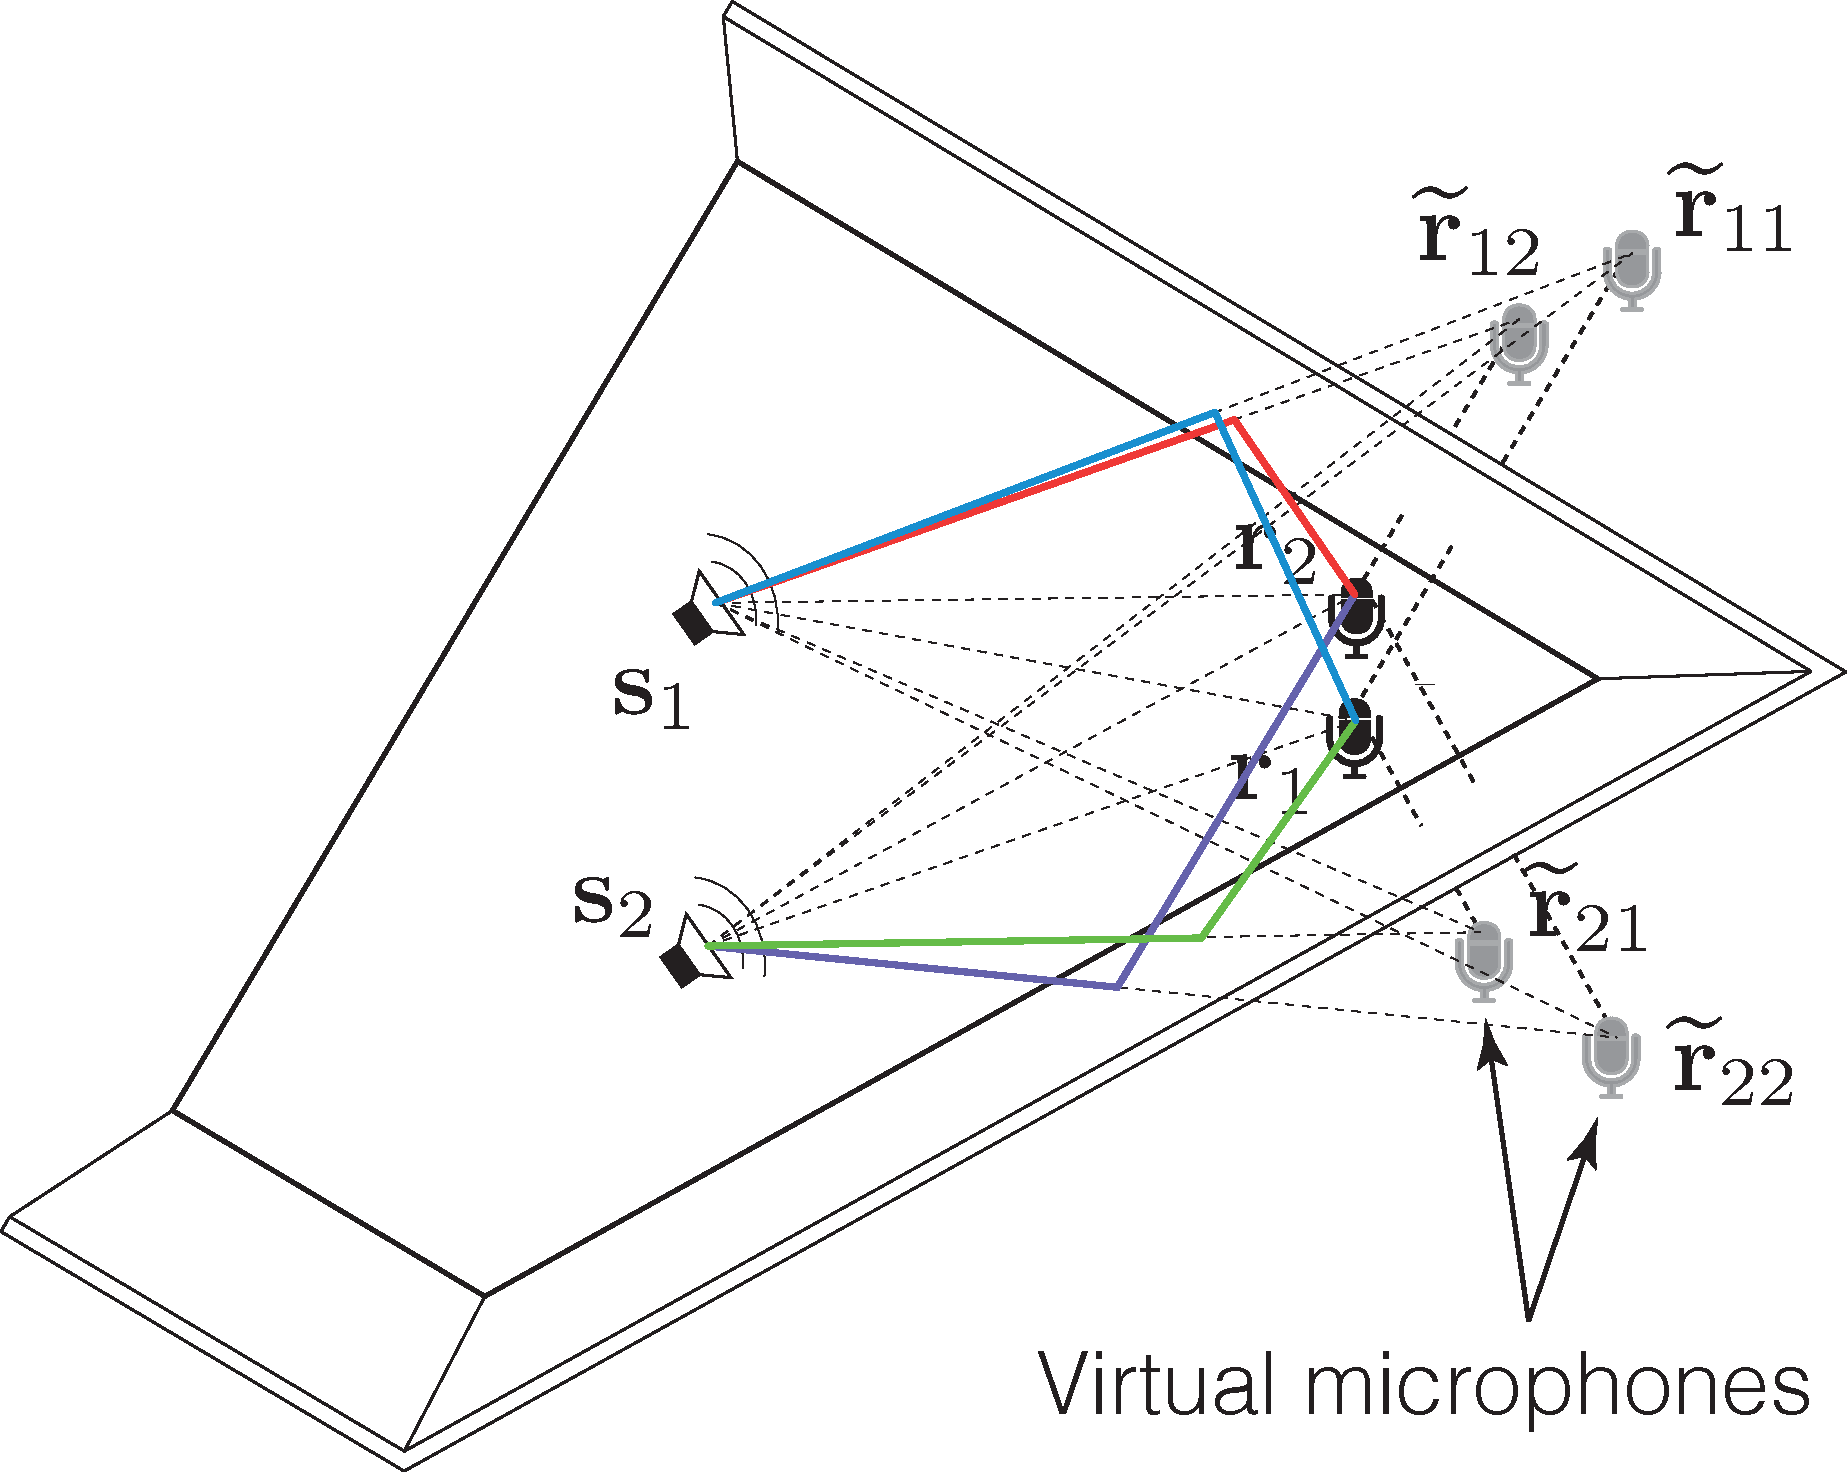
\includegraphics[width=.7\linewidth]{separake/separake.pdf}
    \end{sidecaption}
\end{figure}

\newthought{Traslating echoes to image array} provide a interest physical interpretation in light of beamforming theory.
Real and virtual microphones form dipoles with diverse frequency-dependent directivity patterns.
By integrating more and more virtual microphones the directivity pattern changed and higher spatial selectivity can be achieved~\citeonly{dokmanic2015raking}.
This effect is shown in~\cref{fig:separake:directivity}.
\begin{figure}[h]
    \begin{fullwidth}
    \centering
    \subfloat[mu_spkr][Dipole]{
        \includegraphics[width=0.20\linewidth]{separake/microphones_dipoles_tripoles_2.pdf}
        \label{fig:separake:dipole}
    }%
    \subfloat[mu_spkr][Dipole Beampattern]{
        \includegraphics[width=0.48\linewidth]{separake/rir_dipoles.pdf}
        \label{fig:separake:dipole}}
    \\
    \subfloat[mu_univ][Tetrapole]{
            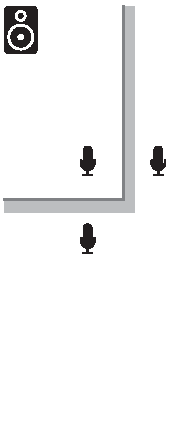
\includegraphics[width=0.20\linewidth]{separake/microphones_dipoles_tripoles_3.pdf}
            \label{fig:separake:tetra}
    }%
    \subfloat[mu_univ][Tetrapole]{
        \includegraphics[width=0.48\linewidth]{separake/rir_tripoles.pdf}
        \label{fig:separake:tetra}}
    \label{fig:separake:results}
    \caption{Frequency-dependent directivity pattern }
    \end{fullwidth}
\end{figure}
Our goal is to design algorithms which benefit from this known spatial diversity.

\subsection{Our Goal and Main Findings}
Our emphasis here is different than that in \citeonly{leglaive2015multichannel}.
Rather than fitting the echo model, we aim to show that separation in the presence of echoes is in fact better than separation without echoes.
We ask the following questions:
\begin{enumerate}
    \item Is speech separation with echoes fundamentally easier than speech separation without echoes?
    Are there specific settings where this is true or false?
    \item Is it necessary to fully model the reverberation or can we get away with a geometric perspective where we know the locations of a few virtual microphones?
\end{enumerate}
To answer these questions we set up several simple experiments.
We take two standard, well-understood multi-channel source separation algorithms which estimate the channel (the \RTFs/),
and instead of updating the channel estimate we simply fix it to the \RTFs/ of real and a few virtual microphones.
The first algorithm---\NMFdef/ via \MU/---only uses the magnitudes of the transfer functions, while the second one---\EMdef/---also uses the phases.
In this initial investigation we look at the (over)determined case ($J \leq M$),
leaving the analysis of the undetermined case to future work. Our findings can be summarized as follows:
\begin{description}
    \item[\MU/] With magnitudes only, multi-channel anechoic separation is hardly any better than single-channel separation:
    as the magnitude of the transfer functions is the same at all microphones, channel modeling offers no diversity.
    The situation is different in rooms where the direction-dependent magnitude of \RTFs/ varies significantly from microphone to microphone.
    We show that replacing the transfer functions with a few echoes (even just one) gives significant performance gains compared to not modeling the \RTFs/ at all,
    but also that it does better than learning the \RTFs/ through multiplicative updates.
    \item[\EM/] With both phases and magnitudes, anechoic separation will be near-perfect since it corresponds to a determined linear system.
    Therefore, any uncertainty from imperfections in channel modeling will make things worse.
    Surprisingly, approximating the \RTFs/ with one echo matches learning them through EM updates and using more outperforms it.
\end{description}

\section{Modeling}
% Let us recall the continuous-time domain signal model presented is~\cref{ch:processing}.
% Suppose $J$ sources emit inside the room and we have $M$ microphones.
% Each microphone receives
% \begin{equation}
%     \tilde{\mic}_\idxMic(t) = \sum_{\idxSrc = 1}^{\numSrcs} \tilde{\img}_{\idxMicSrc}(t),
% \end{equation}
% with $\tilde{\img}_{\idxMicSrc}$ being the spatial image of the $\idxSrc$-th source at the $\idxMic$-th microphone.
% Spatial images are given as
% \begin{equation}
%     \tilde{\img}_{\idxMicSrc}(t) = (\tilde{\src}_\idxSrc \convCont \tilde{\flt}_{\idxMicSrc})(t),
% \end{equation}
% where $\tilde{\flt}_{\idxMicSrc}$ is the room impulse response between the source $\idxSrc$ and microphone $\idxMic$.
% The room impulse response is a central object in this paper.
% We model it as
% \begin{equation}
%     \tilde{\flt}_{\idxMicSrc}(t) = \sum_{\idxEch = 0}^{\numEchs} \alpha_{\idxMicSrc}^{(\idxEch)} \delta(t - \tau_{\idxMicSrc}^{(\idxEch)}) + \tilde{\varepsilon}_{\idxMicSrc}(t),
% \end{equation}
% where the sum comprises the line-of-sight propagation and the earliest $\numEchs$ echoes we want to account for (at most 6 in this paper),
% while the error term $\tilde{\varepsilon}_{\idxMicSrc}(t)$ collects later echoes and the tail of the reverberation.
% We do not assume $\tilde{\varepsilon}_{\idxMicSrc}(t)$ to be known.
% We assume that the sources are in the far field of real and virtual microphones so the times $\tau_{\idxMicSrc}^{(\idxEch)}$ depend only on the source DOAs which we assume are known.

\mynewline
Assuming $\numEchs$ echoes per source are known, we can form an approximate \RTF/ from source $\idxSrc$ to microphone $\idxMic$,
\begin{equation}
    \label{eq:separake:approx_tf}
    \tilde{H}_{\idxMicSrc}(f) = \sum_{\idxEch=0}^{\numEchs} \alpha_{\idxMicSrc}^{(\idxEch)} \cste^{-\csti 2 \pi f \tau_{\idxMicSrc}^{(\idxEch)}}.
\end{equation}
The far field assumption implies that only the relative arrival times are known so we can arbitrarily fix the delay of the direct path to zero.
In addition, we assume all walls to be spectrally flat in the frequency range of interest and that $\alpha_{\idxMicSrc}^{(\idxEch)}$ are known up to a scaling (i.e. $\alpha_{\idxMicSrc}^{(0)} = 1$).
In this work we assume that the echoes properties are known and for their estimation is discussed~\cref{pt:estimation} of this thesis.

\mynewline
Assuming the narrowband approximation, hence, the model presented in \cref{subsec:processing:model:stft}, the \STFTdef/ of the $\idxMic$-th microphone signal reads
\begin{equation}
    \label{eq:separake:stft}
    \MIC_\idxMic[k,l] = \sum_{\idxSrc = 1}^{\numSrcs} H_{\idxMicSrc}[k] \MIC_{\idxSrc}[k,l] + \NSE_\idxMic[k,l]
\end{equation}
with $k$ and $l$ being the frequency and frame index,
$H_{\idxMicSrc}[k]$ is the \DFT/ approximating the \RTF/ of~\eqref{eq:separake:approx_tf},
$\MIC_{\idxSrc}[k,l]$ the \STFT/ of the $\idxSrc$-th source signal, and $\NSE_\idxMic[k,l]$ a term including noise and model mismatch.
It is convenient to group the microphone observations in vector form,
\begin{equation}
    \MICS[k,l] = \FLTSS[k]\SRCS[k,l] + \NSES[k,l].
\end{equation}
where $\MICS[k,l] = \klist{\MIC_\idxMic[k,l]}_\idxMic$,
$\FLTSS[k] = \klist{H_{\idxMicSrc}[k,l]}_{\idxMicSrc}$,
$\SRCS[k,l] = \klist{\SRC_\idxSrc[k,l]}_\idxSrc$,
and $\NSES[k,l] = \klist{\NSE_\idxMic[k,l]}_\idxMic$.

\mynewline
Let the squared magnitude of the spectrogram of the $\idxSrc$-th source be $\mP_\idxSrc = \klist{\powerOf{\MIC_{\idxSrc}[k,l]} }_{kl}$.
The non-negative factor model assume that the spectrogram is a matrix $\mP_\idxSrc$ resulting from a product of 2 non-negative matrices:
\marginpar{
    \centering
    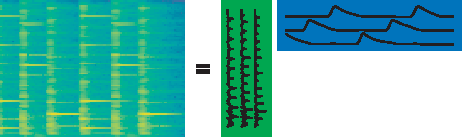
\includegraphics[width=\linewidth]{separake/nmf_example_source.pdf}
    \captionof{figure}{
        Spectrogram of a sound source signal decomposed into dictionary and activation
    }\label{fig:separake:nmf_source}
}
\begin{equation}
    \label{eq:separake:nmf}
    \mP_\idxSrc =  \mD_\idxSrc \mZ_\idxSrc,
\end{equation}
where $\mD_\idxSrc$ is the non-negative \textit{dictionary} whose contains the spectral can be interpreted as spectral templates of the source,
and the latent variables $\mZ_\idxSrc$, called \textit{activations}, indicates when and how this templates are activated.
This is shown in~\cref{fig:separake:nmf_source}.

\newthought{The Audio Source separation} can then be cast as an inference problem in which we maximize the likelihood of the observed $\MICS$ over all possible non-negative factorizations \eqref{eq:separake:nmf}.
This normally involves learning the channels (frequency-domain mixing matrices).
Instead of learning them, we build the channels based on the prior knowledge of the earliest few echoes.

\section{Source Separation by NMF}
To evaluate the usefulness of echoes in source separation, the multi-channel \NMF/ framework of \citeauthor{ozerov2010multichannel}~\citeonly{ozerov2010multichannel}.
Second, rather than learning the \RTF/ from the data, we use the approximate model of \eqref{eq:approx_tf}.
In the following we briefly describe the two algorithms used.

\subsection{NMF using Multiplicative Updates (MU-NMF)}\label{sec:separake:mu}
\MUdef/ for \NMF/ only involve the magnitudes only and the updates rules are guaranteed non-negative as long as the initialization is.
They have been originally proposed by in \citeonly{Lee:2001ti}.
We use the \textit{Itakura-Saito divergence} \citeonly{Fevotte:2011af} between the observed multi-channel squared magnitude spectra $\mV_\idxMic = \klist{\powerOf{\MIC_\idxMic[k,l]}}_{kl}$ and their non-negative factorizations,
\begin{equation}
    \label{eq:mu_nmf}
    \wh{\mV}_\idxMic = \sum_{\idxSrc=1}^{\numSrcs} \diag(\vQ_{\idxMicSrc}) \mD_\idxSrc \mZ_\idxSrc , \quad \idxMic=1,\ldots,\numMics
\end{equation}
\marginpar{
    \centering
    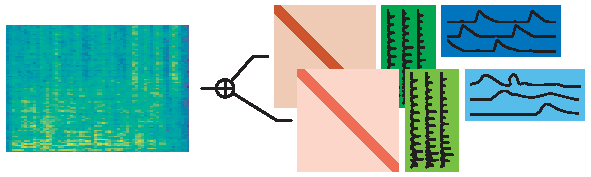
\includegraphics[width=\linewidth]{separake/mu_nmf_signal_model.pdf}
    \captionof{figure}{
        Schematics of the signal model used for \MU/-\NMF/.
    }\label{fig:separake:nmf_mu}
}
where $\vQ_{\idxMicSrc} = \klist{\powerOf{H_{\idxMicSrc}[k]}}_k$ is the vector of squared magnitudes of the approximate \RTF/ between microphone $\idxMic$ and source $\idxSrc$.

\newthought{The MU cost function} is minimize the divergence between the observed spectrogram $(V_{\idxMic}[k,l]$ and the model $\wh{V}_{\idxMic}[k,l]$, that is,
\begin{equation}
    \scrC_{\mathtt{MU}}(\mZ_\idxSrc) = \sum_{\idxSrc k l} \calD_{\mathtt{IS}}(V_{\idxMic}[k,l] | \wh{V}_{\idxMic}[k,l])
    + \gamma \sum_\idxSrc \kvvbar{\mZ_\idxSrc}S_1,
\end{equation}
where $\calD_{\mathtt{IS}}( v | \hat{v} ) = \frac{v}{\hat{v}} - \log \frac{v}{\hat{v}} - 1$.
We add an $\ell_1$-penalty term to promote sparsity in the activations due to the potentially large size of the universal dictionary~\citeonly{Sun:2013co}.

\newthought{The MU updating rule} are obtain by adapting the original \MU/ rule derivations from \citeauthor{ozerov2010multichannel}:
\begin{align}
    \mZ_\idxSrc \gets \mZ_\idxSrc \odot \frac{\sum_\idxMic (\diag(\vQ_{ij}) \mD_\idxSrc)^\top \left(\mV_\idxSrc \odot \wh{\mV}_\idxSrc^{-2}\right)}{\sum_\idxMic(\diag(\vQ_{ij}) \mD_\idxSrc)^\top \wh{\mV}_\idxSrc^{-1} + \gamma},
\end{align}
where multiplication $\odot$, power, and division are element-wise.
\\Importantly, neglecting the reverberation (or working in the anechoic regime) leads to a constant $\vQ_{\idxMicSrc}$ for all $\idxSrc$ and $\idxMic$.
A consequence is that the \MU/-\NMF/ framework breaks down with a universal dictionary.
Indeed, \eqref{eq:mu_nmf} becomes the same for all $\idxMic$,
\begin{equation*}
    \wh{\mV}_\idxMic = \sum_{\idxSrc} \mD \mZ_\idxSrc = \mD \sum_\idxSrc \mZ_\idxSrc,
\end{equation*}
so even with the correct atoms identified, we can assign them to any source without changing
the value of the cost function. Therefore, anechoic multi-channel separation with a universal dictionary cannot work well.
This intuitive reasoning is corroborated by numerical experiments in Section \ref{sec:results}.
Of course, in line with the message of this paper, this problem is overcome by using echoes.


\subsection{NMF using Expectation Maximization (EM-NMF)}\label{sec:separake:em}
Unlike the \MU/ algorithm that independently maximizes the log-likelihood of \RTF/ magnitudes, the \EM/-\NMF/ maximizes the joint log-likelihood over all complex-valued channels~\citeonly{ozerov2010multichannel}.
Hence, the model takes into account observed phases.
Each image source $\idxSrc$ is modeled as the sum of components with complex Gaussian priors of the form $\IMG_{\idxMicSrc}[k,l]\sim \mathcal{N}_c\kparen{0, d_{\idxMicSrc,k}z_{\idxMicSrc,n}}$ such that
\begin{equation}
    \MIC_\idxSrc[k,l] \sim \mathcal{N}_c \kparen{0, (\mD_\idxSrc\mZ_\idxSrc)_{kl}},
\end{equation}
and the magnitude spectrum $\mP_\idxSrc$ of \eqref{eq:separake:nmf} can be understood as the variance of source $\idxSrc$.
\\Under this model, and assuming uncorrelated noise, the microphone signals also follow a complex Gaussian distribution with covariance matrix
\begin{equation}
    \mSigma_{\MICS}[k,l] = \FLTSS[k] \mSigma_{\SRCS} [k,l] \khermitian{\FLTSS}[k] + \mSigma_{\NSES}[k,l].
\end{equation}

\newthought{The \EM/ cost function} correspond to the negative log-likelihood of the observed signal, that is,
\begin{equation}
    \scrC_{\mathtt{EM}}(\mZ_\idxSrc) = \sum\limits_{kl} \trace\kparen{\MICS[k,l] \khermitian{\MICS[k,l]} \mSigma_{\MICS}^{-1}[k,l]} \\
    + \log\det\mSigma_{\MICS}[k,l].
\end{equation}
This quantity can be efficiently minimized using the \EM/ algorithm proposed in~\citeonly{ozerov2010multichannel}.
We modify the original algorithm by fixing the source dictionaries $\mD_\idxSrc$ and the early-echo channel model $\FLTSS[k]$ throughout the iterations.
Since adding sparsity priors is not straightforward in the \EM/ framework, the universal dictionary was left for future work.

\newthought{The \EM/ updating rules} are


\section{Numerical Experiments}

We test our hypotheses through computer simulations.
In the following, we describe the simulation setup, dictionary learning protocols, and we discuss the results.

\subsection{Setup}
An array of three microphones arranged on the corners of an equilateral triangle with edge length $\SI{0.3}{\m}$ is placed in the corner of a 3D room with 7 walls.
We select 40 sources at random locations at a distance ranging from $\SI{2.5}{\m}$ to $\SI{4}{\m}$ from the microphone array.
Pairs of sources are chosen so that they are at least $\SI{1}{\m}$ apart.
The floor plan and the locations of microphones are depicted in Figure~\ref{fig:separake:rir_room}\marginpar{
    \centering
    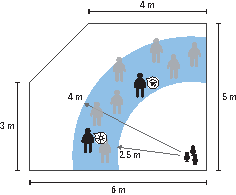
\includegraphics[width=\linewidth]{figures/separake/room_setup}
    \captionof{figure}{
        The simulated scenario.
    }
    \label{fig:separake:rir_room}
}.
The scenario is repeated for every two active sources out of the 780 possible pairs.

\mynewline
The sound propagation between sources and microphones is simulated using the
image source model implemented in \textit{pyroomacoustics} Python package~\citeonly{scheibler2017pyroomacoustics}.
The wall absorption factor is set to $0.4$, leading to a $\RT$ of approximately $\SI{100}{\ms}$.
An example RIR is shown in Figure~\ref{fig:separake:rir_room}.
The sampling frequency is set to $\SI{16}{\kHz}$, \STFT/ frame size to $2048$ samples with $50\%$ overlap between frames, and we use a cosine window for analysis and synthesis.
Partial \RTFs/ are then built from the $\numEchs$ nearest image microphones.
The global delay is discarded, and only the relative amplitudes between echoes are kept.

\mynewline
With this setup, we perform three different experiments.
In the first one, we evaluate MU-NMF with a universal dictionary.
In the other two, we evaluate the performance of \MU/-\NMF/ and \EM/-\NMF/ with speaker-specific dictionaries.
We vary $\numEchs$ from 1 to 6 and use three baseline scenarios:
\begin{enumerate}
\item \textit{anechoic}: Anechoic conditions, no model mismatch.
\item \textit{learn}: The \RTFs/ are learned from the data along the activations as originally proposed~\citeonly{ozerov2010multichannel}.
\item \textit{no echoes}: Reverberation is present but ignored (i.e. $\numEchs=0$).
\end{enumerate}
With the universal dictionary, the large number of latent variables warrants the introduction of sparsity-inducing regularization.
The value of the regularization parameter $\gamma$ was chosen by a grid search on a holdout set with the signal-to-distortion ratio ($\SDR$) as the figure of merit \citeonly{vincent2007first} (Table~\cref{tab:separake:gamma}).

\begin{table}
    \begin{sidecaption}[]{
        Value of the regularization parameter $\gamma$ used with the universal dictionary.
        }[tab:separake:gamma]
        \centering
        \small
        \begin{tabular*}{\linewidth}{@{\extracolsep{\fill}}lccccccccc@{}}
    \toprule
     &       &          & \multicolumn{7}{c}{{\footnotesize Number of echoes $\numEchs$}} \\
     \cmidrule{4-10}
     & anechoic & learn & 0 & 1 & 2 & 3 & 4 & 5 & 6 \\
     \cmidrule{2-10}
     $\gamma = $ & $10$ & $10^{-1}$ & $10$ & $10^{-3}$ & 0 & 0 & 0 & 0 & 0 \\
     \bottomrule
\end{tabular*}
    \end{sidecaption}
\end{table}


\subsection{Dictionary Training, Test Set, and Implementation}
To evaluate the usefulness of echoes in source separation, the multi-channel \NMF/ framework of \citeauthor{ozerov2010multichannel}~\citeonly{ozerov2010multichannel}.
First, we introduce a dictionary learned from available training data.
We explore both speaker-specific and universal dictionaries \citeonly{Sun:2013co}.
Speaker-specific dictionaries can be beneficial when speakers are known in advance.
Universal dictionary is more versatile but gives a weaker regularization prior.

\begin{figure}[h]
    \begin{fullwidth}
    \centering
    \subfloat[mu_spkr][Speaker-specific dictionary]{
        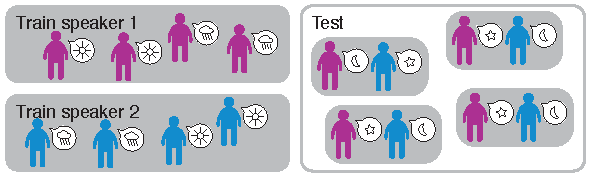
\includegraphics[width=0.48\linewidth]{separake/dict_speaker_dep.pdf}
        \label{fig:separake:dict_spk}}
        \hfill
    \subfloat[mu_univ][Universal dictionary]{
        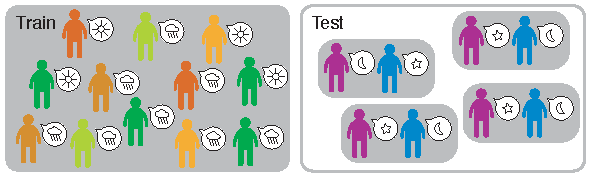
\includegraphics[width=0.48\linewidth]{separake/dict_universal.pdf}
        \label{fig:separake:dict_univ}}
    \label{fig:separake:results}
    \end{fullwidth}
\end{figure}


\newthought{Universal Dictionary:} Following the methodology of \citeonly{Sun:2013co} we select 25 male and 25 female speakers
and use all available training sentences to form the universal dictionary
$
    \mD = [\mD_1^\mathtt{M}\cdots \mD_{25}^\mathtt{M}\,\mD_{1}^\mathtt{F}\cdots\mD_{25}^\mathtt{F}].
$
The test signals were selected from speakers \emph{and} utterances outside the training set.
The number of latent variables per speaker is 10 so that with STFT frame size of 2048 we have $\mD\in\R^{1025\times500}$.

\newthought{Speaker-Specific Dictionary:}
Two dictionaries were trained on one male and one female speaker.
One utterance per speaker was excluded to be used for testing.
The number of latent variables per speaker was set to $20$.

\mynewline
All dictionaries were trained on samples from the TIMIT corpus \citeonly{garofolo1993timit} using the \NMF/ solver in \library{scikit-learn} Python package~\citeonly{pedregosa2011scikit}.

\newthought{Implementation:} Authors of \citeonly{ozerov2010multichannel} provide a Matlab implementation\sidenote{
    \href{http://www.irisa.fr/metiss/ozerov/Software/multi_nmf_toolbox.zip}{Multichannel nonnegative matrix factorization toolbox (in Matlab)}
} of \MU/-\NMF/ and \EM/-\NMF/ methods for stereo separation.
We ported their code to Python and extended it to arbitrary number of input channels\sidenote{
    Our implementation and all experimental code are publicly available in line with the philosophy of reproducible research.
}.
However this software features some ad-hoc decisions which do not fit our scenario.
Thus, we provide a Python3 adaptation with the following modifications.
\begin{itemize}
    \item First the original code was restricted to the 2-channel case, i.e.  $\numMics = 2$.
    Thus, in order to embrace the specifics of our scenario and for sake of generalization, we extend it to the multi-channel case, that is $\forall \numMics \geq 1$.
    \item the \MU/-\NMF/ was modified to handle sparsity constraint as described in \ref{sec:separake:mu}.
    \item since \EM/ method degenerates where zero-valued entries are present in the dictionary matrix, $\mD$, all these entries are initially set to a small constant value of $10^{-6}$.
    \item the code was further modified to deal with fixed dictionary and channel models matrices, which are normalized in order to avoid indeterminacy issues \citeonly{ozerov2010multichannel}.
\end{itemize}
Now to conclude with, no \textit{simulated annealing} strategies are not used in the final experiments.
In fact in some preliminary and informal investigations we noticed that this yields to better results then using annealing.
In the experiments, the number of iterations for \MU/-\NMF/ (\EM/-\NMF/) was set to $200$ ($300$).

\subsection{Results}
\label{sec:results}

We evaluate the performance in terms of signal-to-distortion ratio (\SDR) and source-to-interference ratio (\SIR) as defined in \citeonly{vincent2007first}.
We compute these metrics using the \library{mir\_eval} toolbox~\citeonly{raffel2014mir_eval}.

\begin{figure}[t]
    \begin{fullwidth}
    \centering
    \subfloat[mu_univ][MU-NMF, Universal dictionary]{
        \includegraphics[width=0.32\linewidth]{separake/20171025-111558_5ae4058906_near_wall_mu_UnivDict_violin_plot.pdf}
        \label{fig:separake:mu_univ}}
    \hfill
    \subfloat[mu_spkr][MU-NMF, Speaker-specific dictionary]{
        \includegraphics[width=0.32\linewidth]{separake/20171026-192746_360771b8ce_near_wall_mu_SpkrDict_violin_plot.pdf}
        \label{fig:separake:mu_spkr}}
    \hfill
    \subfloat[em_spkr][EM-NMF, Speaker-specific dictionary]{
        \includegraphics[width=0.32\linewidth]{separake/20171027-050909_e9d8c07aef6_near_wall_em_SpkrDict_violin_plot.pdf}
        \label{fig:separake:em_spkr}}
    \caption{Distribution of SDR and SIR for male and female speakers as a function of the number of echoes included in modeling, and comparison with the three baselines.}
    \label{fig:separake:results}
    \end{fullwidth}
\end{figure}


\begin{figure}[th]
    \begin{sidecaption}[]{
            Summary of the median SDR and SIR for the different algorithms evaluated.
            \label{fig:separake:median}
        }[fig:separake:median]
        \centering
        \small
        \includegraphics[width=\linewidth]{separake/all_medians.pdf}
    \end{sidecaption}
\end{figure}

\mynewline
The distributions of \SDR and \SIR for separation using \MU/-\NMF/ and a universal dictionary are shown in \cref{fig:separake:mu_univ}, with a summary in \cref{fig:separake:median}.
We use the median performance to compare the results from different algorithms.
First, we confirm that separation fails for flat \RTFs/ (\textit{anechoic} and $\numEchs=0$) with \SIR at around 0~dB.
Learning the \RTFs/ performs somewhat better in terms of \SIR than in terms of \SDR, though both are low.
Introducing approximate \RTFs/ dramatically improves performance: the proposed approach outperforms the learned approach even with a single echo.
With up to six echoes, gains are +2~dB \SDR and +5~dB \SIR.
Interestingly, with more than one echo, $\ell_1$ regularization becomes unnecessary; non-negativity and echo priors are sufficient for separation.

\mynewline
Separation with speaker-dependent dictionaries is less challenging since we have a stronger prior.
Accordingly, as shown in ~\cref{fig:separake:mu_spkr,fig:separake:median}, \MU/-\NMF/ now achieves a certain degree of separation even without the channel information.
The gains from using echoes are smaller, though one echo is still sufficient to match the median performance of learned \RTFs/.
Using an echo, however, results in a smaller variance.
Adding more echoes further improves \SDR{} (\SIR) by up to +2~dB (+3~dB).

\mynewline
In the same scenario, \EM/-\NMF/ (\cref{fig:separake:em_spkr}) has near-perfect performance on anechoic signals which is expected as the problem is overdetermined.
For \MU/, a single echo suffices to reach the performance of learned \RTFs/ and further improve it.
Moreover, echoes significantly improve separation quality as illustrated by up to 3~dB improvement over \textit{learn}.
It is interesting to note that in all experiments the first three echoes near-saturate the metrics.
This is good news since higher order echoes are hard to estimate.

%\begin{itemize}
%    \item Universal dictionary scenario: Here, the speakers are unknown.
%    \begin{itemize}
%        \item Because the MU method does not use phase and hence no time delay information across channels, source separation in the anechoic scenario is impossible. Here, we see that using reverberated signals instead with knowledge of only a few echoes significantly improve source separation performance: up to +2dB SDR and +5 dB SIR.
%        \item Using a fixed echo model for channels also outperform learning the channels, even with a single echo.
%        \item Note that EM could not be used for the universal dictionary scenario, because the corresponding model is not designed to handle dictionaries with hundreds of atoms. A sparsity-enforcing Bayesian prior on the estimated activation Z would need to be included, which is not straightforward.
%        \item Increasing the number of known echoes beyond 3 does not bring significant improvement.
%    \end{itemize}
%    \item Speaker-dependent dictionary scenario. This scenario is on the one hand easier because speakers are known and on the other hand harder because much less training data is used, allowing much fewer atoms to represent speech in the dictionaries.
%    \begin{itemize}
%        \item Unsurprisingly, EM performs extremely well in the anechoic setting. This is because perfect knowledge of the complex-valued over-determined mixing filters is then available, through the time differences of arrival. Results would likely be very different in an under-determined setting, where perfect filter knowledge is not enough to separate signals.
%        \item Once again, it is showed that using knowledge of a few echoes significantly improve results with respect to an anechoic model, up to +2dB SDR and +3dB SIR for both methods.
%        \item EM performs slightly better (+1.5 dB) than MU in terms of SIR, suggesting that modeling the phase of mixing filters help.
%        \item In this scenario, knowledge of the echoes starts significantly outperforming the baseline (the learned model) when 3 echoes are known (+3dB SIR).
%        \item Again, increasing the number of known echoes beyond 3 does not bring significant improvement.
%    \end{itemize}
%\end{itemize}

\section{Conclusion}

In this paper we began studying the role of early echoes in sound source separation---a challenging task in computational auditory scene analysis.
We found that a simple echo model not only improves performance, but it also enables separation in conditions where it is otherwise not possible.
One such example is separation with non-negative speaker-independent models.
Echoes seem to play an essential role in magnitude-only algorithms like non-negative matrix factorization via multiplicative updates.
They improve separation as measured by the standard metrics even when compared to approaches that learn the transfer functions.
We believe these results are only a first step in understanding the potential of echoes in computational auditory scene analysis.
They suggest that simple models used in this paper could be used as regularizers in other common audio processing tasks.
Ongoing work includes running real experiments, studying the underdetermined case, and blindly estimating the wall parameters.

%Future work:
%\begin{itemize}
%    \item Update the late-reverberation part of mixing matrices in EM
%    \item Adding sparsity priors to activations to use larger dictonary with EM
%    \item Experiments with more microphone/room configurations, more sources
%    \item Use a DOA estimation algorithm to infer the early echo models.
%    \item Estimate the absorption factors of nearby surfaces.
%\end{itemize}